\documentclass[a4paper, 11pt]{report}
\usepackage[a4paper,margin=1in]{geometry}
\usepackage{dirtree}
 \usepackage[at]{easylist}
\usepackage[utf8]{inputenc}
\usepackage{graphicx}
\usepackage{hyperref}
\usepackage{fancyhdr}
\graphicspath{ {./Figures/} }
\usepackage[table,xcdraw]{xcolor}
\usepackage{listings}
\usepackage{xcolor}
\usepackage{cite}

\definecolor{codegreen}{rgb}{0,0.6,0}
\definecolor{codegray}{rgb}{0.5,0.5,0.5}
\definecolor{codepurple}{rgb}{0.58,0,0.82}
\definecolor{backcolour}{rgb}{0.95,0.95,0.92}
\setlength{\headheight}{13.6pt}
\newenvironment{simplechar}{%
   \catcode`\$=12
   \catcode`\&=12
   \catcode`\#=12
   \catcode`\^=12
   \catcode`\_=12
   \catcode`\~=12
   \catcode`\%=12
}{}

\lstdefinestyle{mystyle}{
    backgroundcolor=\color{backcolour},   
    commentstyle=\color{codegreen},
    keywordstyle=\color{magenta},
    numberstyle=\tiny\color{codegray},
    stringstyle=\color{codepurple},
    basicstyle=\ttfamily\footnotesize,
    breakatwhitespace=false,         
    breaklines=true,                 
    captionpos=b,                    
    keepspaces=true,                 
     numbers=left,                    
    numbersep=5pt,                  
    showspaces=false,                
    showstringspaces=false,
    showtabs=false,                  
    tabsize=2
}

\lstset{style=mystyle}


\fancypagestyle{plain}{
  \fancyhf{}% Clear header/footer
  \rhead{John Montgomery - 5199}
\lhead{Kimberley College - 15162}
\lfoot{\thepage}
\rfoot{Robotron 2084: Pygame remake}
}
\pagestyle{plain}% Set page style to plain.

\title{%
    
    \begin{center}
        
\includegraphics[width=3cm]{kimberley.png}
        \centering
    \end{center}
  Robotron: 2084 inspired Game \\
  \large Written in PyGame with MVC architecture}
\author{{\Large John Montgomery}\\ \ 
Candidate Number: 5199\\
Centre Name: Kimberley College\\
Centre Number: 15162\\
Qualification: AQA 7517 (A--Level Computer Science)\\ \\
{\small Supervisor: B. Harris}}
\date{2020-2022}




\begin{document}

\maketitle

\newpage
\tableofcontents\thispagestyle{empty}
\newpage
\listoffigures\thispagestyle{empty}
\newpage
\chapter{Abstract}
    This project is a modernised version of robotron 2084, it has 2 sections, the game code and the website. The game code, which is a remake of Robotron 2084, a classic arcade game, this is backed with an MVC architecture which is designed to separate out the functionalities of the game and communicates with the website via an API. The website will use a database with multiple tables to store all the scores and logins and will also be used to display the high scores of users.

\chapter{Analysis}
    \section{Introduction}
The goal of this project was to create a more modernised version of Robotron: 2084, the classic arcade game from the 80s. In order to make it a more modern version I will make a few additions, including improving the game itself and increase the competition aspect of it. I also needed to modernise the codebase itself, and couldnt build off the existing code written in the 80s.

As i was unable to access the code from the original game, nor find a viable method to emulate the code on my machine, i was forced to take my research from websites, videos and images, and whilst this isnt ideal, i was still able to gain a vast amount of information and replicate the game how i wanted to.

Whilst there is no specific target audience for the project, it could be played and enjoyed by anyone, ranging from my classmates to the people who played and enjoyed the original game from the 80s. Thanks to the wide range of possible users, there is a large market i can test this app with.

\section{About the game}

Robotron 2084 is a classic, top down, arcade game from the 80's, in which, a player (who is a mutant genetic super hero) attempts to save the last human family from swarms of killer robots. The game was a 2 stick shooter originally - this means 2 joysticks, one to move and one to shoot (this allows the 2 to occur individually and simultaneously). This was one of the first of its kind, and was largely considered a success. The game has a number of waves with varying number or robots, of different types, and varying numbers of humans.

In order to 'save' a human, they player simply has to touch them, this rescues the human and scores the player points. The more humans saved, the higher the points. The player, whilst a mutant, is still susceptible to damage - and whilst there is no 'health' the player can be killed rather easily. The robots simply have to touch the player (or the player accidentally collide with them) and the player 'dies'. You start the game with 3 lives and slowly progress through the waves - a new wave starts when all of the grunts (one of the robots, see table below) are killed, or when the player dies. 
There are also various transition screens, including a boot screen, a testing screen and end screens. Along with these come a live counter, a score counter and flashing borders. The game is fast passed and bright, and graphically complex, with lots of colours and intense action. Making a game like this play as smoothly as they did at the time was truly an accomplishment.
The game even had sound! whilst it was only mono aural (no stereo) - this was still impressive, considering it was a game running on a 1MHz processor. They were able to develop this in a 2 man team over a period of 6 months. It was itself heavily influenced by a number of other games, including 'Berzerk' - a shooting game which players traverse a maze and shoot at enemies. However, this was a single stick shooter (with a button to fire) rather than a dual stick shooter.
The game had sequels but none were as successful as the original, and were never received as well. One even attempted a multiplayer system, where one would shoot and another would move, but this was not widely seen as a positive update.

\section{More Modern 2D games}
In order to bring this game into the 21st century, it will need more modernised features. For one, almost everyone plays games on computers, and as such, will need a 'dual stick' implementation. Almost every modern game uses WASD to move and arrows to shoot, but IJKL is also used to shoot. Other approaches to avoid seeming like a single stick shooter are using the mouse to control movement or shooting, or even ESDX and IJKM as move and shoot (this was the original set up for Robotron 2084 on apple products. 

\section{Robotron's Design}
I mostly used video for my research into robotrons design - this felt like the best way due to how fast the game changes, with fast animations and colour changes, something that cannot be captured easily in photo screenshots. I also relied on websites, also linked, for more technical information and this is where i was also able to learn lots of the history behind the game.


\begin{itemize}
    \item \url{https://www.youtube.com/watch?v=ccltMtkFBSI} - This video - impressive in itelf for the gameplay, gave me more of an insight into the feel of the past paced nature of the game, and whilst the quality isnt perfect, it gives some idea of the general layout of the screen and game
    
    \item \url{https://www.youtube.com/watch?v=aOVA2Axxfdk} - This video was much higher quality screen capture of the game, this is what allowed me to see animation and character design as well as have a very good understanding of what layouts looked like, and the general interface.
    
    \item \url{https://arcadeblogger.com/2020/06/27/the-development-of-robotron/} This was possibly my most used resource. Having insight into the development and original views of the game was very important, and this website alone would probably have been enough to implement it. 
\end{itemize}

Whilst i didn't want to build a carbon copy of the original, i did endeavour to create something as similar as i could without loosing too much of the fast paced nature of the game.


\section{Robotron Step by Step}
Robotron starts up with a pattern of random pixels, followed by a screen indicating that tests were successful (or, as it may be, unsuccessful), before finally transitioning to the start screen. This screen has the words Robotron, along with credits to the developer. It is very bright, and flashing. The game also has a high score board displaying at the end of every run (and i believe it would also display at times when the machine was not in game). When starting the game, it would show a level transition screen (bright rectangles would display from the centre of the screen moving out). A wave would then start. This would begin by displaying all character, but not allowing movement of enemies for a few moments (this is probably a design choice, a brief moment for the player to plan their first few movements, and analyse where they should head). The levels would then loop like this, with a transition showing between each.

To illustrate the game layout better, i have included a finite state machine of how the game would work, it can be found below in \ref{fig:Robotron FSM}.

\begin{figure}[ht!]
  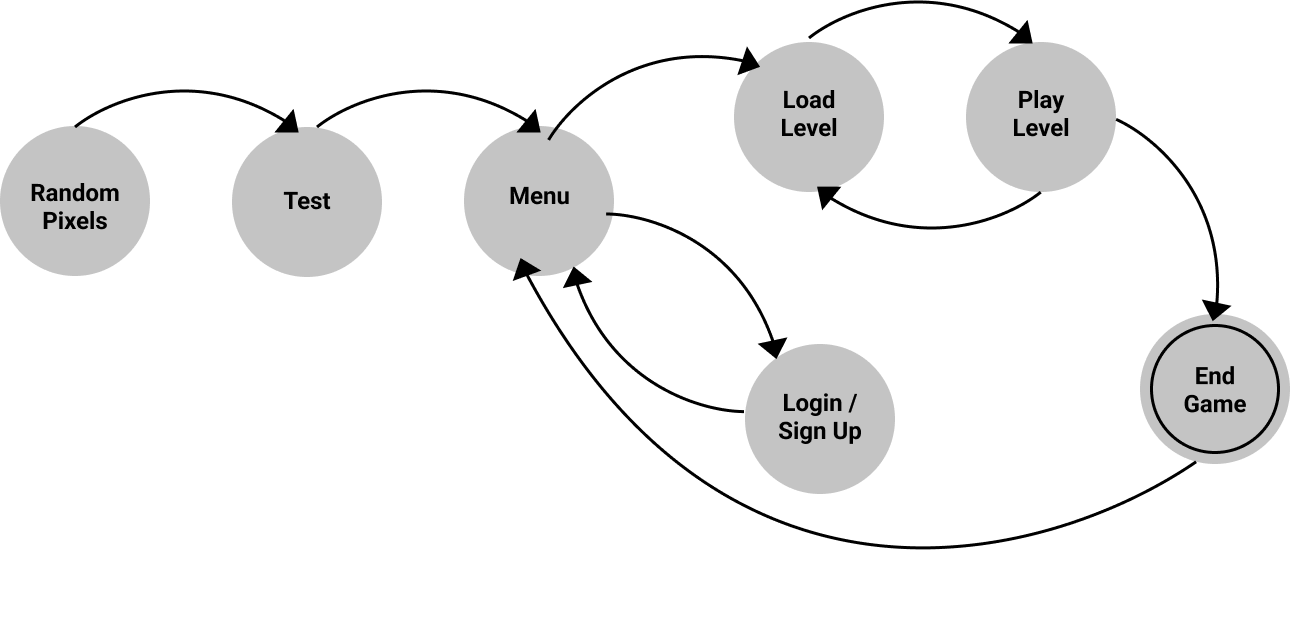
\includegraphics[width=0.8\linewidth]{Figures/FSM_robotrom.png}
  \centering
  \caption{The FSM which shows a very basic overview of how robotron 2084 works}
  \label{fig:Robotron_FSM}
\end{figure}


\section{Enemy Specific Behaviour}
One problem with not having access to the original code is the inability to tell what algorithm was used to cause the grunt enemy to 'flock' to the player (the only enemy I will implement which is actively seeking to get to the player) there are a few ways i could have done this, almost all of them much more simple than the method I would end up on.

A very basic approach to creating something like this is to simply move in the direction of the player, at a speed of x pixels per blit. This would have lead to some issues though. The main one being crowding. This would allow lots of grunts to 'stack', making it easier to kill them (a stream of bullets into this stack, and they are all destroyed). As such, this was rejected. I considered adding a random element to this (like having them move at a random speed, or adding some random direction) - but this would risk the grunts becoming jittery.

The solution is to use an algorithm called 'boids'. It is known as an artificial life program, and is meant to mimic the flocking of birds (boids = bird-oid object). It works by applying individual rules to each boid (each item in the flock) which results in a hive mind sort of intelligence. It is made up of 3 basic rules, plus 1 more to allow the group to move towards the goal (in this case the player).

\subsection{Rule 1 - move to centre mass}
First, calculate the centre of mass, for the boids in view. Essentially, sum all x and y co ordinate values and divide by the number of boids, for the co ordinates of the centre (c) $(\frac{\Sigma x}{n_{boids}},\frac{\Sigma y}{n_{boids}})$. Then, we want to move the boid 1\% of the way towards this centre, so our actual movement vector is given by $\frac{c - P_{boid}}{100}$ (where $P_{boid}$ is the position of the currently calculated boid), we need to subtract $P_{boid}$ as we want to move 1\% of the distance from the current position, not from the position $(0,0)$.
    
\subsection{Rule 2 - Avoid collisions with other boids}
This one is much more simple. For this, we simply want to move away from the other boids. To do that, just add the magnitudes of the difference between the 2 current positions to get a new position. 

\subsection{Rule 3 - Match velocities of the other boids}
This is also somewhat complex but works like Rule 1. We want to have the boids attempt to match the velocities of the boids around it. This could be done with some similar maths. First, sum all the velocities (V) $(\frac{\Sigma V_x}{n_{boids}},\frac{\Sigma V_y}{n_{boids}})$, much like with Rule 1, we dont want to match this velocty perfectly. Instead, add about a twentieth of the calculated value, which can be performed with $\frac{V - V_{boid}}{20}$

\subsection{Rule 4 - Move towards the player}
This rule is easy. Find the distance to the player, and move about a 5th of the way there.

\subsection{Notes on boids}
I did not create the boids flocking algorithm. It was created by Craig Reynolds, \url{http://www.red3d.com/cwr/boids/} is where i pulled most of my information from. This is a tweaked version from the original, with altered values that i set to perform more how i wanted (eg, to emulate a hoard of robots over flocking birds) and with the added rule of moving towards a player. 

\section{Python Library selection}
I had to select python libraries to handle 2 large sections of my code, these were the web framework and the gui framework. These both are hugely popular areas of python development, and there are a multitude of frameworks which i would have used, but there were 2 major contenders for each.

\subsection{Web Framework Library}
This was a relatively simple choice, flask or django. I had already decided that this would be a relatively simple website with a need for a larger focus to the API, and less need for web content. As such, django makes less sense, and flask is much faster, so this was quite an easy solution to use. In the past I've also found flask easier to deploy and debug, certainly it was my preference of backend anyway - but it also made sense.

\subsection{GUI Library}
Python has a few possible libraries, but again, 2 main contenders. TkInter and PyGame. TkInter is built in, and i have used it in the past, but when I used it, I used it for fairly basic forms, and at most, a chess game. These were no fast paced, and I wasnt convinced it would handle the huge number of sprites and fast moving objects. As such, I decided to go with Pygame, which is much better suited to this.

\section{Game Code Architecture}
Selecting an architecture was important. It was clear from the get go that this project would heavily use OOP, as it made sense, not just for sprites in general but also for its ease of use with pygame. I could have had a very simple system with a game loop and processing in there. I eventually settled on a specific design, and that was MVC (Model-View-Controller) as an architecture for the game.  This divides the logic into 3 components, 1, the model, which handles all the data, and is esentially the 'backend' of the game; 2, the view, this is the part the user sees, and is fed from the model, and finally, the controller, which is how the user interacts with the machine, and this feeds the model. 

For example, whilst it may have been possible to have it so that whenever a WASD key is pressed, the view is instantly moved to show the updated position - MVC dictates that you first update the model, and then on the next blit this update gets drawn up. This may seem somewhat counter intuative, but means each component can be swapped out much easier, leading to an incredibly modular design. This makes it much easier to develop, improve and test.

The system will also use a state machine (implemented with a stack) to control what is currently shown on screen as each state has its own meaning and definitions of what is needed on screen. Again, this allows for a much more modular system, as individual functions can be called once the current state is identified. It will also have an event system - such that it is a largely data driven system, where data is processed on the fly as it is received.

\section{Objectives}
\begin{easylist}[articletoc]
@ Game Objectives
@@ Main (hero) character objectives
@@@ Character can be displayed
@@@ Character can move in all 8 directions
@@@ Character faces in correct direction
@@@ Characters movement is animated
@@@ Character is bounded to window
@@@ Character can shoot in 8 directions
@@@ Player is invincible on load of level
@@ Enemy character objectives (for each enemy type - Electrodes, Grunts and Hunks)
@@@ Enemies can be displayed
@@@ Enemies can move
@@@ Enemy faces correct direction
@@@ Enemies movement is animated
@@@ Enemy are bounded to window
@@@ Enemy kills player when touching
@@@ Specific enemy functionality
@@@@ Electrodes are randomly spread around the page
@@@@ Grunts flock around player
@@@@ Hunks slow down when shot
@@ Menu objectives
@@@ Logo is shown and animated
@@@ Display static text
@@@ Display animated text
@@@ Display and allow input for options
@@@ Allow for login and sign up
@@ Extras objectives (additional features) 
@@@ Flashing border
@@@ Random colour load screen
@@@ "All tests" screen
@@@ Inter---level animation
@@@ Sounds
@@@@ For shooting
@@@@ For start up
@@@@ For level change

@ Website Objectives
@@ Displays high score board of top 10 players
@@ Website animated and looks like the high score board on original game
@@ Have an error page, informs user something went wrong
@@ API Goals (a route to...)
@@@ Return top scores
@@@ Allow for sign up
@@@ Allow for log in
@@@ Generate tokens for login
@@@ Upload scores and validate with token
\end{easylist}


\section{What is MVC?}
Model-View-Controller plays a large part in the project, the diagram [Figure \ref{fig:MVC_overview}] shows the main way that MVC works. It isolates the components of the game into 3 main components. The View, which is the screen, or what the user will see. The controller, which is where the user interacts with the game, in this case it is the interaction with the keyboard. The model, which is the part the user never interacts with, and stores the state of the game and current information about it.

\begin{figure}[ht!]
  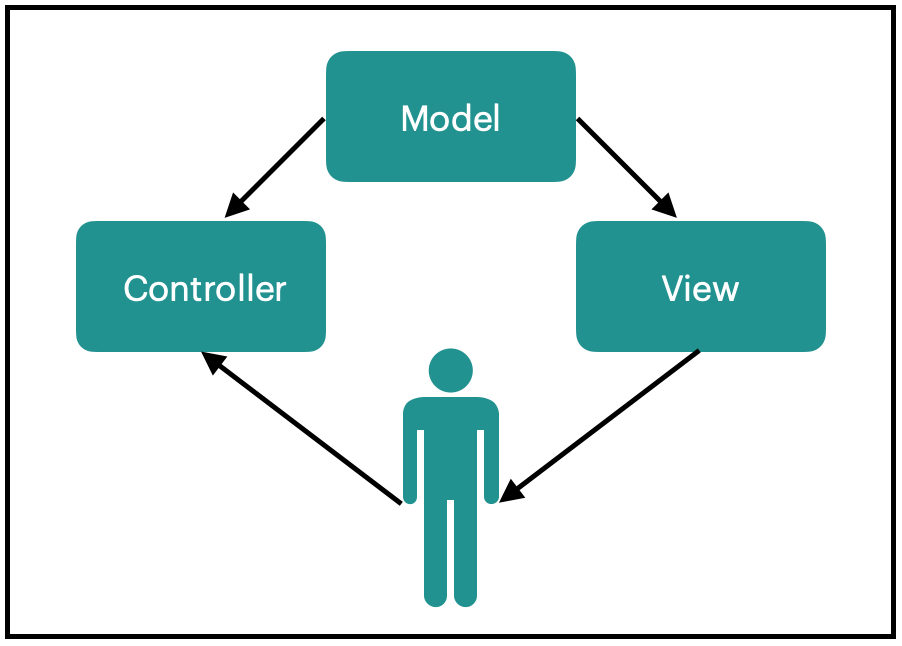
\includegraphics[width=\linewidth]{MVC overview.png}
  \caption{A diagram showing the MVC architecture}
  \label{fig:MVC_overview}
\end{figure}

There are many benefits to this set up, for example, it will easily allow me to swap out what controller is used. If desired, it is much simpler to replace the keyboard as the human interface, and replace it with a game controller. Even more useful may be the ability to remove the controller and view entirely, allowing for a streamlined game which an AI could learn how to play. This flexibility, along with ease of programming is what drew me to use MVC for the game.

Another important information is the way information travels between the 3 sections. This is done with events, and an event manager is responsible for maintaining the sending and receiving of events through the system. A similarly important section is the States, and state machine, which controls the current ‘state’ the game is in, that is to say what level is being played, or what screens should be shown, such as a loading or help screen.

\section{The Game}
“Robotron: 2084” was released in 1982 by Williams Electronics. It was revolutionary as a dual stick shooter, was high energy and loved by many. This is important to capture into the game, where I want it to have a similar feeling to the original game, with some modern twists. 

The game is about a species of ‘Robotrons’ created by humans in the year 2084, after realising their failings and created an advanced species. The goal is to save the humans (Mommies, Daddies and Mikeys), whilst fighting the robots, which have many kinds. The most basic are electrodes, which are static obstacles that kill on contact, but can be shot by players. The other basic enemy is the grunt, which is simply a basic soldier, which kills on contact, but moves towards the player.
There are some other robots that will be talked about and implemented later, but the details about them are less important. 

\section{Limitations}
The dual stick shooter nature means the player uses one joystick to move, and one joystick to shoot. This is difficult to implement well with a keyboard, but a simple setup which I am using is having WASD to move, and IJKL to shoot. Holding 2 keys diagonally at the same time will result it movement in an angle, allowing for shooting in 8 directions, and moving in 8 too.

Robotron is a fast fast game, I had to slow it down slightly in order to make it more playable on my laptop, and so it does feel somewhat different to the original. However by slowing it as I have I have made it a much smoother game to play.

\section{Objectives}
\begin{easylist}[articletoc]
@ Game Objectives
@@ Main (hero) character objectives
@@@ Character can be displayed
@@@ Character can move in all 8 directions
@@@ Character faces in correct direction
@@@ Characters movement is animated
@@@ Character is bounded to window
@@@ Character can shoot in 8 directions
@@@ Player is invincible on load of level
@@ Enemy character objectives
@@@ Enemies can be displayed
@@@ Enemies can move
@@@ Enemy faces correct direction
@@@ Enemies movement is animated
@@@ Enemy can move
@@@ Enemy kills player when touching
@@@ Specific enemy functionality
@@@@ Electrodes are randomly spread around the page
@@@@ Use boids flocking algorithm to dictate movement of grunts
@@@@ Hunks slow down when shot
@@ Menu objectives
@@@ Logo is shown and animated
@@@ Display static text
@@@ Display animated text
@@@ Display and allow input for options
@@@ Allow for login and signup
@@@ Show help menu
@@ Decorations objectives
@@@ Flashing border
@@@ Random colour load screen
@@@ "All tests" screen
@@@ Inter---level animation

@ Website Objectives
@
\end{easylist}

\begin{enumerate}

    \item Create the API
    \item Create login system
        \begin{enumerate}
            \item Basic API sign up works
            \item GUI interactions with PyGame
        \end{enumerate}
    \item High Scores
        \begin{enumerate}
            \item Top 10
            \item Player Search
        \end{enumerate}
    \item Create sounds with Game
    \item Create scoring and score counter
    \item Create a life counter
    \item Automate testing on API and basic functions in PyGame
\end{enumerate}

\section{Design and Inspiration}
The design for all the game is heavily taken from the original game. I used many places to research this, but below is a selection of screenshots and videos which were used in the creation of the game.
\begin{figure}[ht!]
  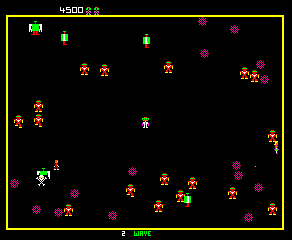
\includegraphics[width=0.8\linewidth]{design1.png}
  \centering
  \caption{Screen from original game - \url{https://arcadeblogger.com/2020/06/27/the-development-of-robotron/}}
  \label{fig:Design 1}
\end{figure}

\begin{figure}[ht!]
  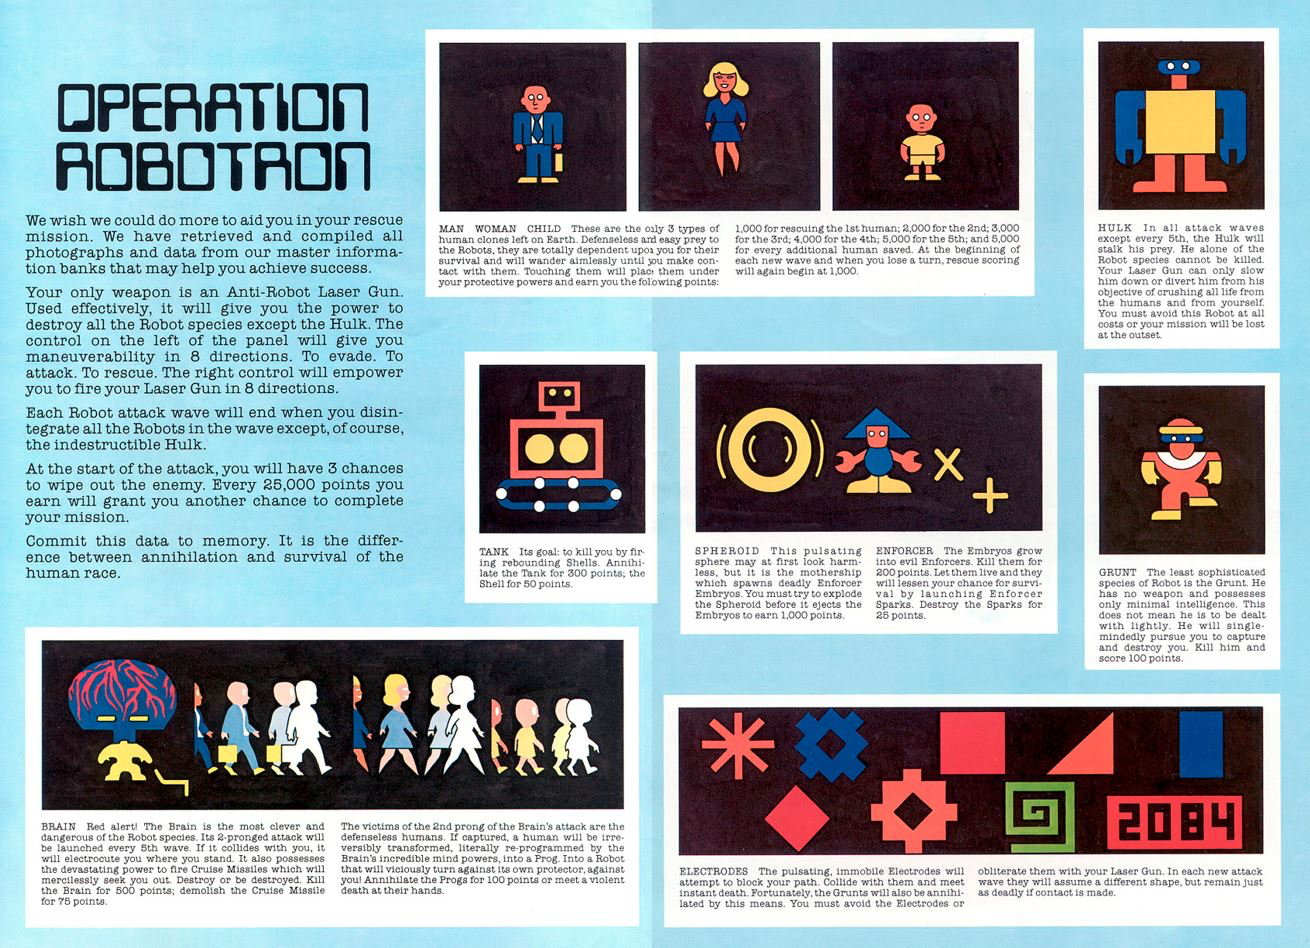
\includegraphics[width=0.8\linewidth]{design2.png}
  \centering
  \caption{Advertising Material - \url{https://arcadeblogger.com/2020/06/27/the-development-of-robotron/}}
  \label{fig:Design 2}
\end{figure}

\begin{itemize}
    \item \href{Video of screenplay, also useful to help create sound}{https://www.youtube.com/watch?v=ccltMtkFBSI}
    
    \item \href{Video of screenplay, also useful to help create sound}{https://www.youtube.com/watch?v=aOVA2Axxfdk}
\end{itemize}



\chapter{Documented Design}
The main design aspect is the MVC architecture and how it forms the basis of the game. Fig 1, from the analysis section, gave a very brief, high level and non technical view of MVC. In this section I will go into more detail about my own implementation, and how it works in greater detail. This section also details the database on the web side, the API, the technical setup of the servers, the data structures and HCI designs.

\section{MVC in practice}
In the analysis section I gave a very high level overview of MVC, this part will detail further into my design on its implementation in python. The first main, basic components of MVC are of course, the model, the view, and the controller. Figure \ref{fig:MVC_class} shows the 3 classes diagrams for each of the implementations of these in python.

\begin{figure}[!ht]
  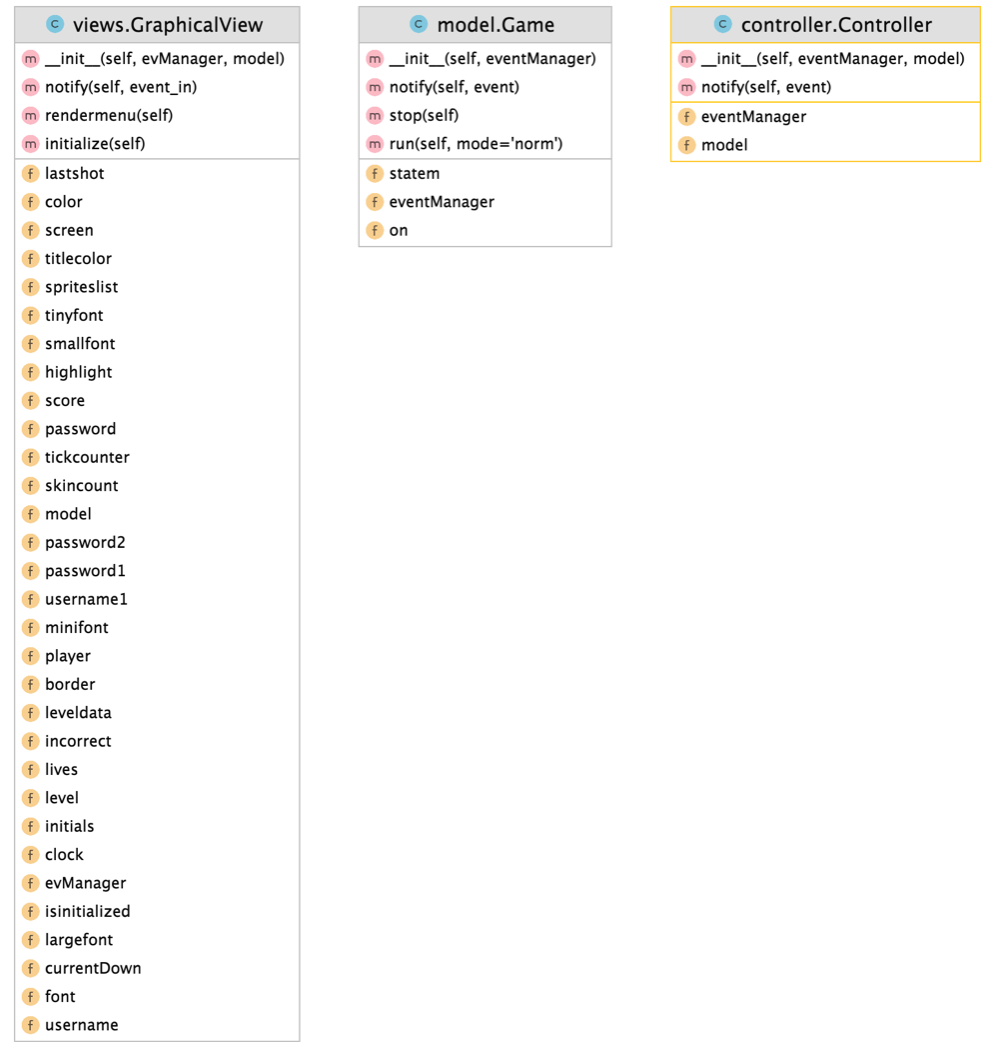
\includegraphics[width=0.8\linewidth]{mvc.png}
  \centering
  \caption{Class diagram}
  \label{fig:MVC_class}
\end{figure}

On top of these key features, there’s also a range of other important cogs in the system. One of the most important, to allow for the communication between the M, V and C are Events, and an event manager. A Sample of events, and the event manager is given in Fig {fig:events}.

\begin{figure}[!ht]
  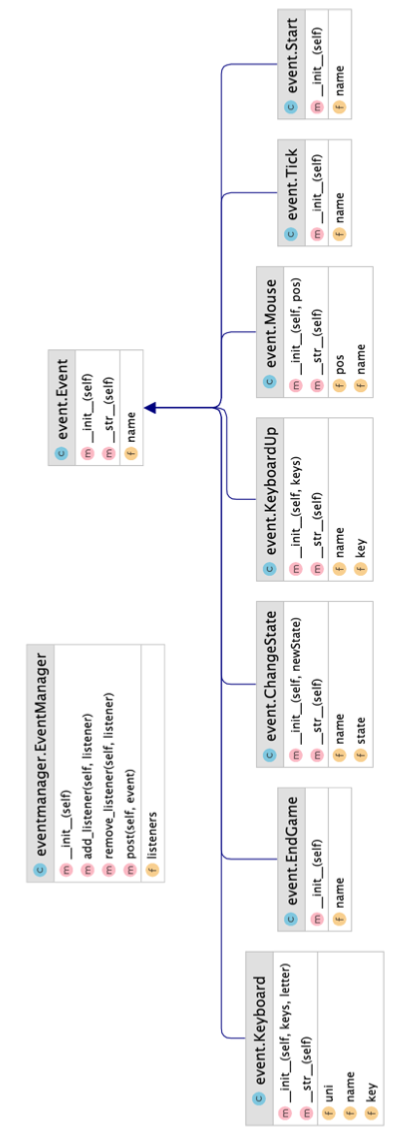
\includegraphics[height=0.8\linewidth, angle=270]{events.png}
  \centering
  \caption{Class diagram}
  \label{fig:events}
\end{figure}

The other key class is the state machine. Each state is not given its own class, rather there is a constant number which is attributed to a given state. The states are used for the larger changes in the program and events are for the smaller interactions, and ticks.
\begin{figure}[!ht]
  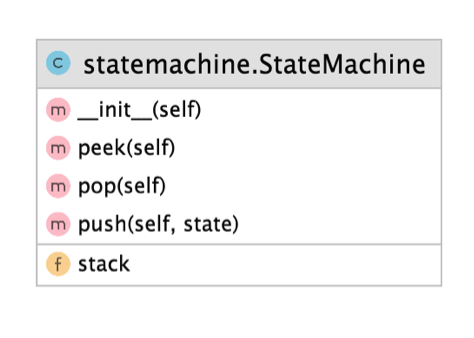
\includegraphics[width=0.8\linewidth]{state.png}
  \centering
  \caption{Class diagram}
  \label{fig:MVC_class1}
\end{figure}

\begin{figure}[!ht]
  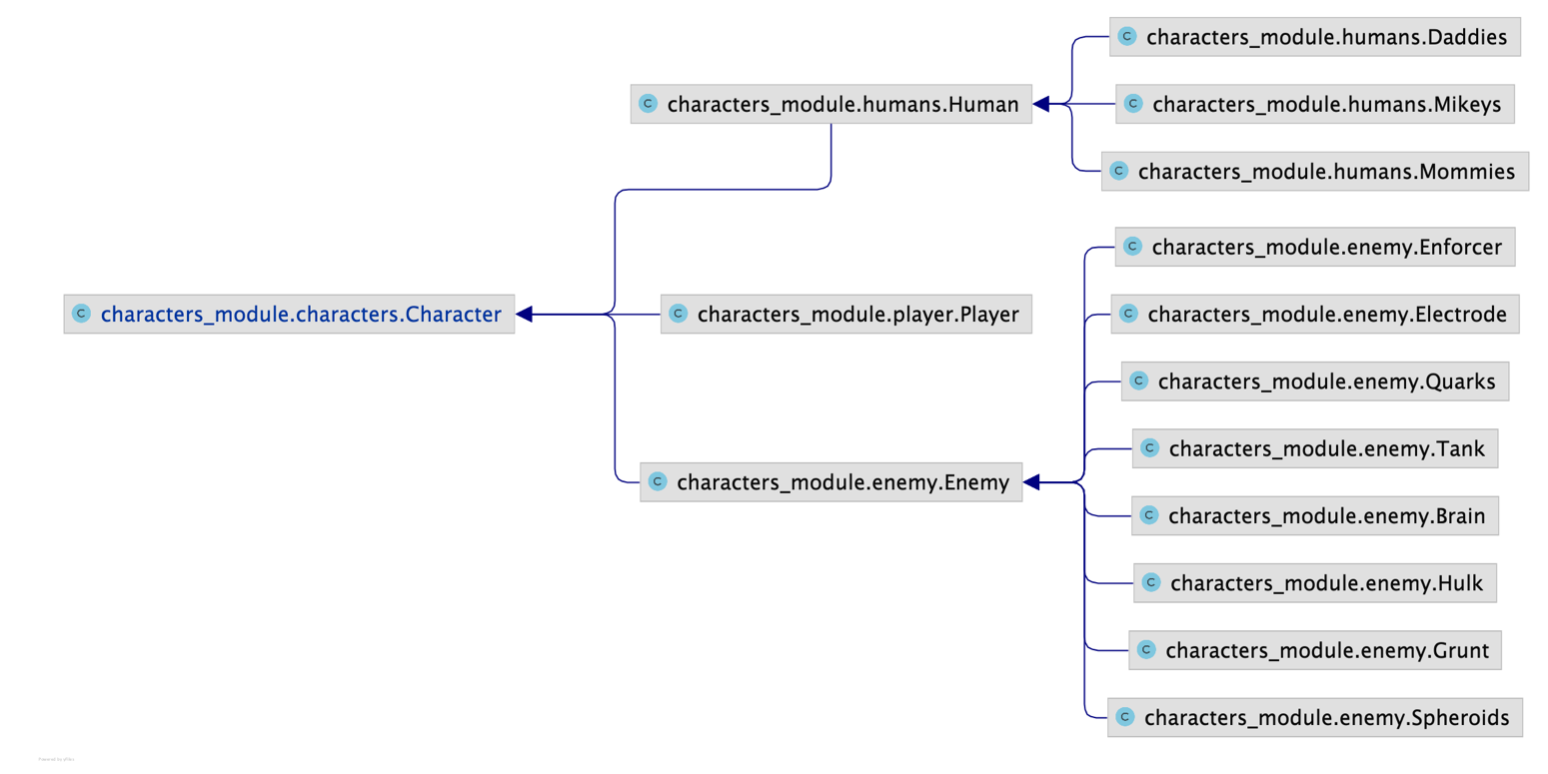
\includegraphics[width=0.8\linewidth]{class2.png}
  \centering
  \caption{Class diagram of characters}
  \label{fig:classeschars}
\end{figure}

\begin{figure}[!ht]
  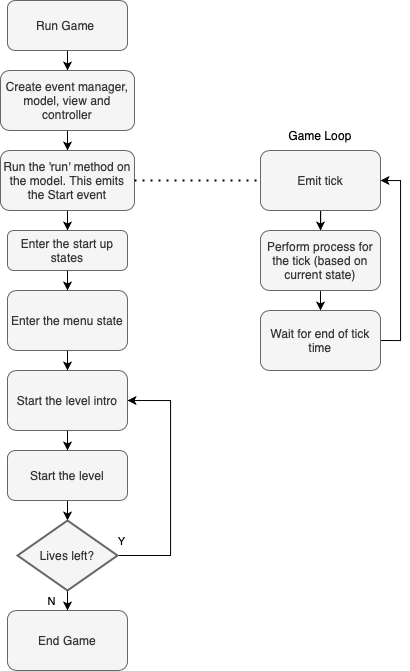
\includegraphics[width=0.8\linewidth]{flowchart}
  \centering
  \caption{Flowchart of MVC}
  \label{fig:flowchart}
\end{figure}

In order to run through a basic idea of what happens when the program is run, I have created a step by step flowchart. This flowchart [Fig 9] is a gross oversimplification, but works as a high level description of what it is my code is doing when executed.

\section{Boids}
I have decided to implement a boids flocking algorithm into the game, this is a mathematical approach to natural flocking behaviour, and whilst this is not the 'AI' used by the robots in the original game (this was closed source, or at least, i have not found it), it does work quite well. Essentially there are 3 rules:

    - move towards the centre of mass of the flock
    - match velocities with the flock
    - avoid collisions
    
in order to make them flock towards the player a 4th rule is added such that, in every iteration, the flock moves slightly closer to the player. This boids algorithm is much better than my original method, which essentially only implemented rule 4, and would get too close to the player and stack.



\section{Database}
This section will show the database design and set up, and explain some of the SQL used in the program. Fig 10 shows the database diagram.


[TODO - Database diagram]


There are 3 tables, scores, users and tokens. The scores database has 2 fields which store the users ID and their Score for a given game. The Users table stores the users info, such as emails, password hashes, etc, and then the tokens database is used to store validated tokens (with time limits) which are used to validate the GUI and avoids needing to login to the the program every time the game is run. Fig 11 shows the process of creating the tokens.

\section{The API}
The leaderboard contains only 6 routes, as these were all that are necessary, the details for the routes are detailed in the table below.

\begin{figure}[!ht]
  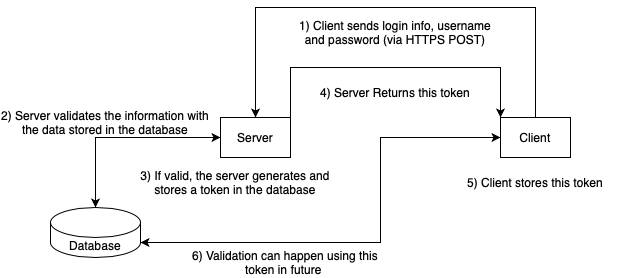
\includegraphics[width=0.8\linewidth]{tokens.png}
  \centering
  \caption{How tokens are generated}
  \label{fig:tokens}
\end{figure}

\begin{table}[!ht]
\begin{tabular}{|l|l|l|}
\hline
\rowcolor[HTML]{C0C0C0} 
ROUTE            & METHOD & DESCRIPTION                                                  \\ \hline
/leaderboard     & GET    & Returns JSON of top 10 users (initials + scores) in Database \\ \hline
/user/userid     & GET    & Returns JSON of top score                                    \\ \hline
/username/userid & GET    & Returns ID of given username                                 \\ \hline
/login           & POST   & Logs in a user, sends token, or logs user in with token      \\ \hline
/addscore        & POST   & Adds a score, given score and a token                        \\ \hline
/adduser         & POST   & Adds a user to the database                                  \\ \hline
\end{tabular}
\end{table}


\section{The Server Setup}
Fig 12 shows the set up the server is in. All using AWS, there is an RDS Postgres database, and EC2 instance (this is the server running the actual flask) and then an S3 bucket to handle sending the static files. It may also be possible to use NGINX or Apache to serve and handle the API. This system may end up being better, so my current architecture could change. 

\section{Security}
Because the database and client handles personal details like email and passwords, there needs to be a thought to security. First off, there is an enforcement of passwords and a strong policy. Users passwords will need to be 8 characters, with 1 special, and my plan is to check them against a list of common passwords (rocky.txt) using hashes. For this I will probably use MD5, or something even faster. However it is important to avoid these fast algorithms when hashing passwords for storage. As such, passwords will undergo key derivation through bcrypt, an algorithm which not only salts, but performs many rounds of hashing. I could implement a similar algorithm using the basic functions like SHA, but rolling your own crypto is never good, so its going to be done with bcrypt, as this is essentially the best option available, and more than secure enough.

To help further security, HTTPS is being used for all the sending and receiving of data, this avoids man in the middle attacks of the data as it gets sent over the internet. 


\chapter{Technical Solution}
Check listings (in the appendix) for a view of all the code. This code is commented to a high standard, but particularly vital sections will be outlined below.

\section{Boids}
Boids was talked about in design, here is the implementation:

First step is creating the function and and setting variables
\lstinputlisting[language=Python, firstline=121, lastline=131]{"Game Code/gameplay.py"}

Now we start looping through each grunt (each member of the flock), and checking if it is 'in view' of the current (x) grunt, to do this, calculate the distance between the points and check less than 60 (eg, a grunt has a sight radius of 60) 
\lstinputlisting[language=Python, firstline=132, lastline=138]{"Game Code/gameplay.py"}

If the boid is in sight then we update our values
\lstinputlisting[language=Python, firstline=139, lastline=144]{"Game Code/gameplay.py"}

then update these values to reflect the centre of the flock etc
\lstinputlisting[language=Python, firstline=145, lastline=150]{"Game Code/gameplay.py"}

these last lines calculate and return the final v of the boid (given as $\Delta x, \Delta y$), which can be added to the current position for the new position.
\lstinputlisting[language=Python, firstline=150, lastline=155]{"Game Code/gameplay.py"}

Now we use some functional type programming to efficiently find and update all the positions
\lstinputlisting[language=Python, firstline=155, lastline=165]{"Game Code/gameplay.py"}



\chapter{Testing - TODO}
\chapter{Evaluation - TODO}

\chapter{Appendix \& Bibliography}
\section{Appendix}
\begin{table}[!ht]
\begin{tabular}{|l|l|l|}
\hline
\rowcolor[HTML]{C0C0C0} 
{\color[HTML]{000000} \textbf{Name}} & {\color[HTML]{000000} \textbf{Server/Web/Game/Dev}} & {\color[HTML]{000000} \textbf{Use}}             \\ \hline
Flask                                & Server                                              & Handles the API and web on server side          \\ \hline
SQLalchemy                           & Server                                              & Used to connect to the Postgres database        \\ \hline
BCrypt                               & Server                                              & Key derivation                                  \\ \hline
Waitress                             & Server                                              & WSGI server                                     \\ \hline
PyGame                               & Game                                                & Graphics and input handling                     \\ \hline
S3                                   & Server                                              & AWS static file hosting / serving               \\ \hline
EC2                                  & Server                                              & AWS server to run flask app                     \\ \hline
Hetzner                              & Server                                              & Alternative option to run flask and serve files \\ \hline
PyCharm                              & Dev                                                 & My IDE choice                                   \\ \hline
\end{tabular}
\section{Bibliography}
\bibliographystyle{apalike}
\bibliography{NEA}


\end{table}
\section{Files and Listings}
This section will outline the file structure of the project, see the file structure diagram of both the game and website code below

\large{Game Code}
TODO INSERT DIR TREE


\large{Website Code}
TODO INSERT DIR TREE

\lstlistoflistings
\subsection{Website Code}

app.py
\lstinputlisting[language=Python]{"Website Code/app.py"}

index.html
\lstinputlisting[language=HTML]{"Website Code/templates/index.html"}

error.html
\lstinputlisting[language=HTML]{"Website Code/templates/error.html"}

styles.css
\lstinputlisting[language=HTML]{"Website Code/static/css/styles.css"}


\subsection{Game Code}

main.py
\lstinputlisting[language=Python]{"Game Code/main.py"}

eventmanager.py
\lstinputlisting[language=Python]{"Game Code/eventmanager.py"}

statemachine.py
\lstinputlisting[language=Python]{"Game Code/statemachine.py"}

model.py
\lstinputlisting[language=Python]{"Game Code/model.py"}

views.py
\lstinputlisting[language=Python]{"Game Code/views.py"}

controller.py
\lstinputlisting[language=Python]{"Game Code/controller.py"}

event.py
\lstinputlisting[language=Python]{"Game Code/event.py"}

states.py
\lstinputlisting[language=Python]{"Game Code/states.py"}

menu.py
\lstinputlisting[language=Python]{"Game Code/menu.py"}

gameplay.py
\lstinputlisting[language=Python]{"Game Code/gameplay.py"}

APIinteractions.py
\lstinputlisting[language=Python]{"Game Code/APIinteractions.py"}

\subsubsection{characters\_module}
characters.py
\lstinputlisting[language=Python]{"Game Code/characters_module/characters.py"}
enemy.py
\lstinputlisting[language=Python]{"Game Code/characters_module/enemy.py"}

humans.py
\lstinputlisting[language=Python]{"Game Code/characters_module/humans.py"}

player.py
\lstinputlisting[language=Python]{"Game Code/characters_module/player.py"}

sprites.py
\lstinputlisting[language=Python]{"Game Code/characters_module/sprites.py"}

\subsubsection{constants}

colors.py
\lstinputlisting[language=Python]{"Game Code/constants/colors.py"}

const.py
\lstinputlisting[language=Python]{"Game Code/constants/const.py"}

\subsubsection{decorations}
border.py
\lstinputlisting[language=Python]{"Game Code/decorations/border.py"}

\subsubsection{objects}
bullet.py
\lstinputlisting[language=Python]{"Game Code/objects/bullet.py"}

\end{document}

